% !TeX root = ../main.tex
\section{问题一的敏感性与有限总体检验}
\label{sec:q1-sensitivity}

\subsection{检验设计}

问题一的主要风险有两类：结论可能对置信水平高度敏感；总体量较小时，二项独立抽样近似可能偏离无放回抽样。为此，分别进行单因素置信水平扰动和有限总体情景分析。改变一个置信水平时保持 $p_0=0.10$ 及另一置信水平为题目给定值，观察相应方向首次存在判定域的样本量；改变 $N$ 时保持两类信度不变，观察超几何模型的统一样本量 $n_*$。本节所有 $N$ 均为检验网格，不是题面数据。

\subsection{置信水平的影响}

表~\ref{tab:q1-confidence-sensitivity}与图~\ref{fig:q1-confidence-sensitivity}给出置信水平扰动结果。

\begin{table}[H]
  \centering
  \caption{置信水平对方向性最小样本量的影响}
  \label{tab:q1-confidence-sensitivity}
  \begin{tabular}{cccc}
    \toprule
    拒收信度 & 首次拒收样本量 & 接收信度 & 首次接收样本量 \\
    \midrule
    $0.900$ & $1$ & $0.80$ & $16$ \\
    $0.925$ & $2$ & $0.85$ & $19$ \\
    $0.950$ & $2$ & $0.90$ & $22$ \\
    $0.975$ & $2$ & $0.95$ & $29$ \\
    $0.990$ & $2$ & $0.99$ & $44$ \\
    \bottomrule
  \end{tabular}
\end{table}

\begin{figure}[H]
  \centering
  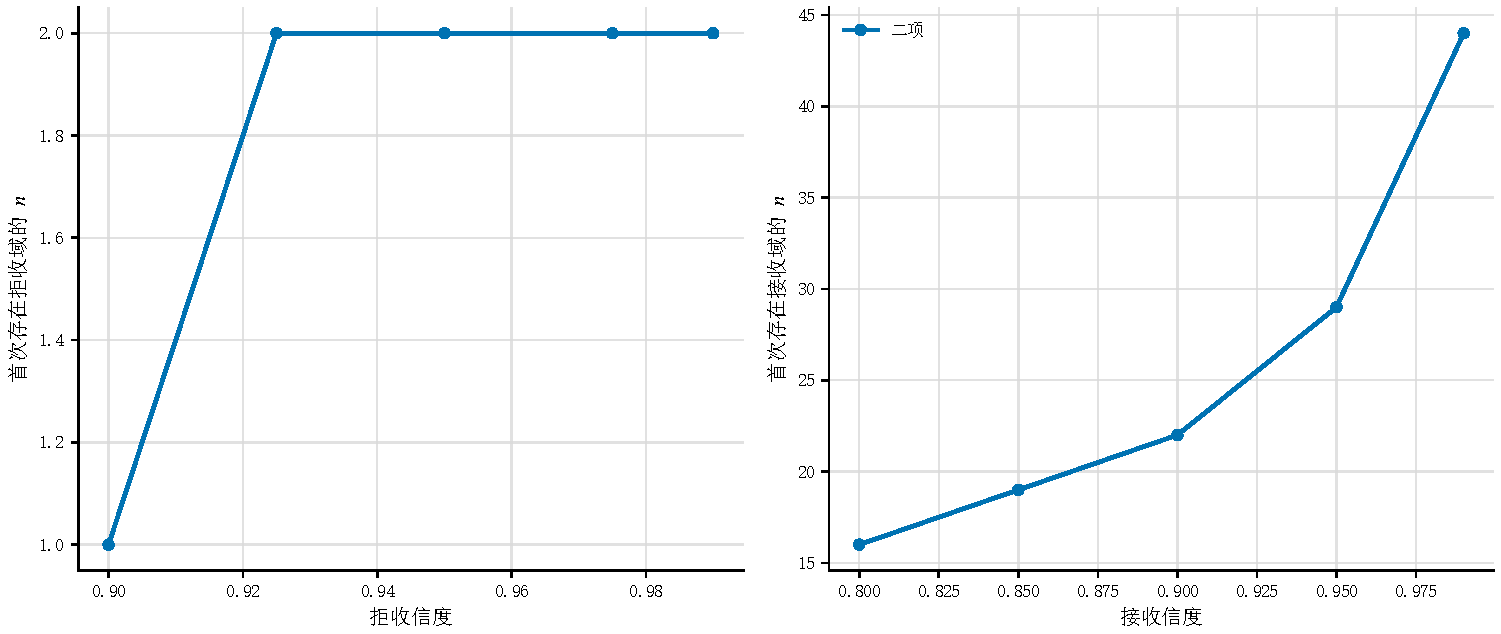
\includegraphics[width=0.96\textwidth]{../../figures/q1/q1_confidence_sensitivity.pdf}
  \caption{置信水平变化对方向性最小样本量的影响}
  \label{fig:q1-confidence-sensitivity}
\end{figure}

接收信度由 $0.80$ 提高到 $0.99$ 时，首次能够接收的样本量由 $16$ 增至 $44$，说明接收样本量对置信水平较为敏感。接收方向需要用很少的次品数排除 $p\ge p_0$ 的情形，信度越高，必须积累越多无次品证据。拒收方向的方向性样本量变化较小，是因为该指标只要求存在一个极端拒收结果，并不衡量一般不合格批次的检验功效。因此，不能把 $n_R=1$ 或 $2$ 单独解释为充分的统一方案。

\subsection{有限总体量的影响}

表~\ref{tab:q1-population-sensitivity}与图~\ref{fig:q1-population-sensitivity}比较不同有限总体量下的超几何统一样本量及二项极限。

\begin{table}[H]
  \centering
  \caption{有限总体量对超几何统一样本量的影响}
  \label{tab:q1-population-sensitivity}
  \begin{tabular}{rrrr}
    \toprule
    $N$ & $D_0=\lfloor0.1N\rfloor$ & 超几何模型 $n_*$ & 相对二项模型差值 \\
    \midrule
    $25$ & $2$ & $13$ & $-9$ \\
    $50$ & $5$ & $16$ & $-6$ \\
    $100$ & $10$ & $18$ & $-4$ \\
    $200$ & $20$ & $20$ & $-2$ \\
    $500$ & $50$ & $21$ & $-1$ \\
    $1000$ & $100$ & $22$ & $0$ \\
    $5000$ & $500$ & $22$ & $0$ \\
    \bottomrule
  \end{tabular}
\end{table}

\begin{figure}[H]
  \centering
  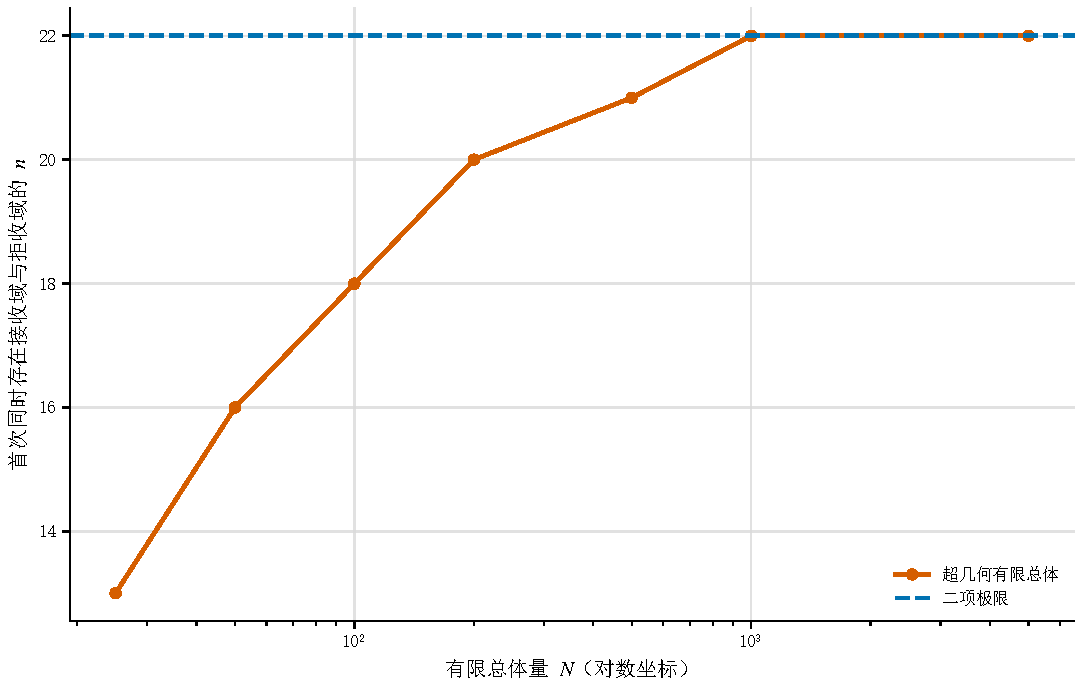
\includegraphics[width=0.88\textwidth]{../../figures/q1/q1_population_sensitivity.pdf}
  \caption{有限总体量变化下超几何模型与二项极限的比较}
  \label{fig:q1-population-sensitivity}
\end{figure}

总体量较小时，抽样占总体的比例较高，无放回抽样提供了更多总体组成信息，因而所需样本量小于二项模型结果。随着 $N$ 增大，有限总体修正逐渐减弱；当 $N=1000$ 和 $5000$ 时，本组参数下 $n_*=22$，与二项模型一致。该趋势支持在总体量较大或抽样比例较低时使用二项模型，而小批次应优先采用超几何精确计算。

\subsection{检验结论}

两组检验表明，统一方案中的接收侧样本量会随置信要求明显变化，不能在改变信度后继续沿用 $n=22$；有限总体量增大时，超几何结果则收敛到二项结果。该结论限定在本节给定参数网格内，不据此声称模型对所有参数扰动均保持稳定。无论采用何种参数，样本量和临界值均应在抽样前确定，并继续保留证据不足区域。
